% !TeX root = thesis.tex
\chapter{Introduction}

\section{Background}
\noindent Drug discovery is slow, expensive, and uncertain. Many candidate drugs fail before they reach the market~\cite{cbo2021rnd}. One reason is that drug effects are hard to predict. A drug may bind to one target protein, but the final response depends on many connected genes, proteins, and signaling pathways inside the cell~\cite{Brown_2025, AnnualReviews_2025}. These systems are highly connected. This makes it hard to predict how a drug changes the state of a cell. Better prediction can therefore help researchers screen compounds earlier and focus on more promising candidates.

\noindent The AstraZeneca ``compound 12'' case, reported in 2025, shows this problem clearly. Figure~\ref{fig:compound_12_inhibitor_mechanism} gives a simple illustration. The compound was designed to act on KRAS, but later analysis suggested that it also affected unintended targets and caused toxic effects in animal studies~\cite{DrugHunter_2025}. The case shows an important point. A drug may reach its intended target and still lead to an unwanted outcome. Its effect can spread through a larger molecular system. This thesis studies that broader prediction problem. The goal is to predict how gene expression changes after drug treatment, relative to a matched control, in a specific cell type.

\begin{figure}[H]
    \centering
    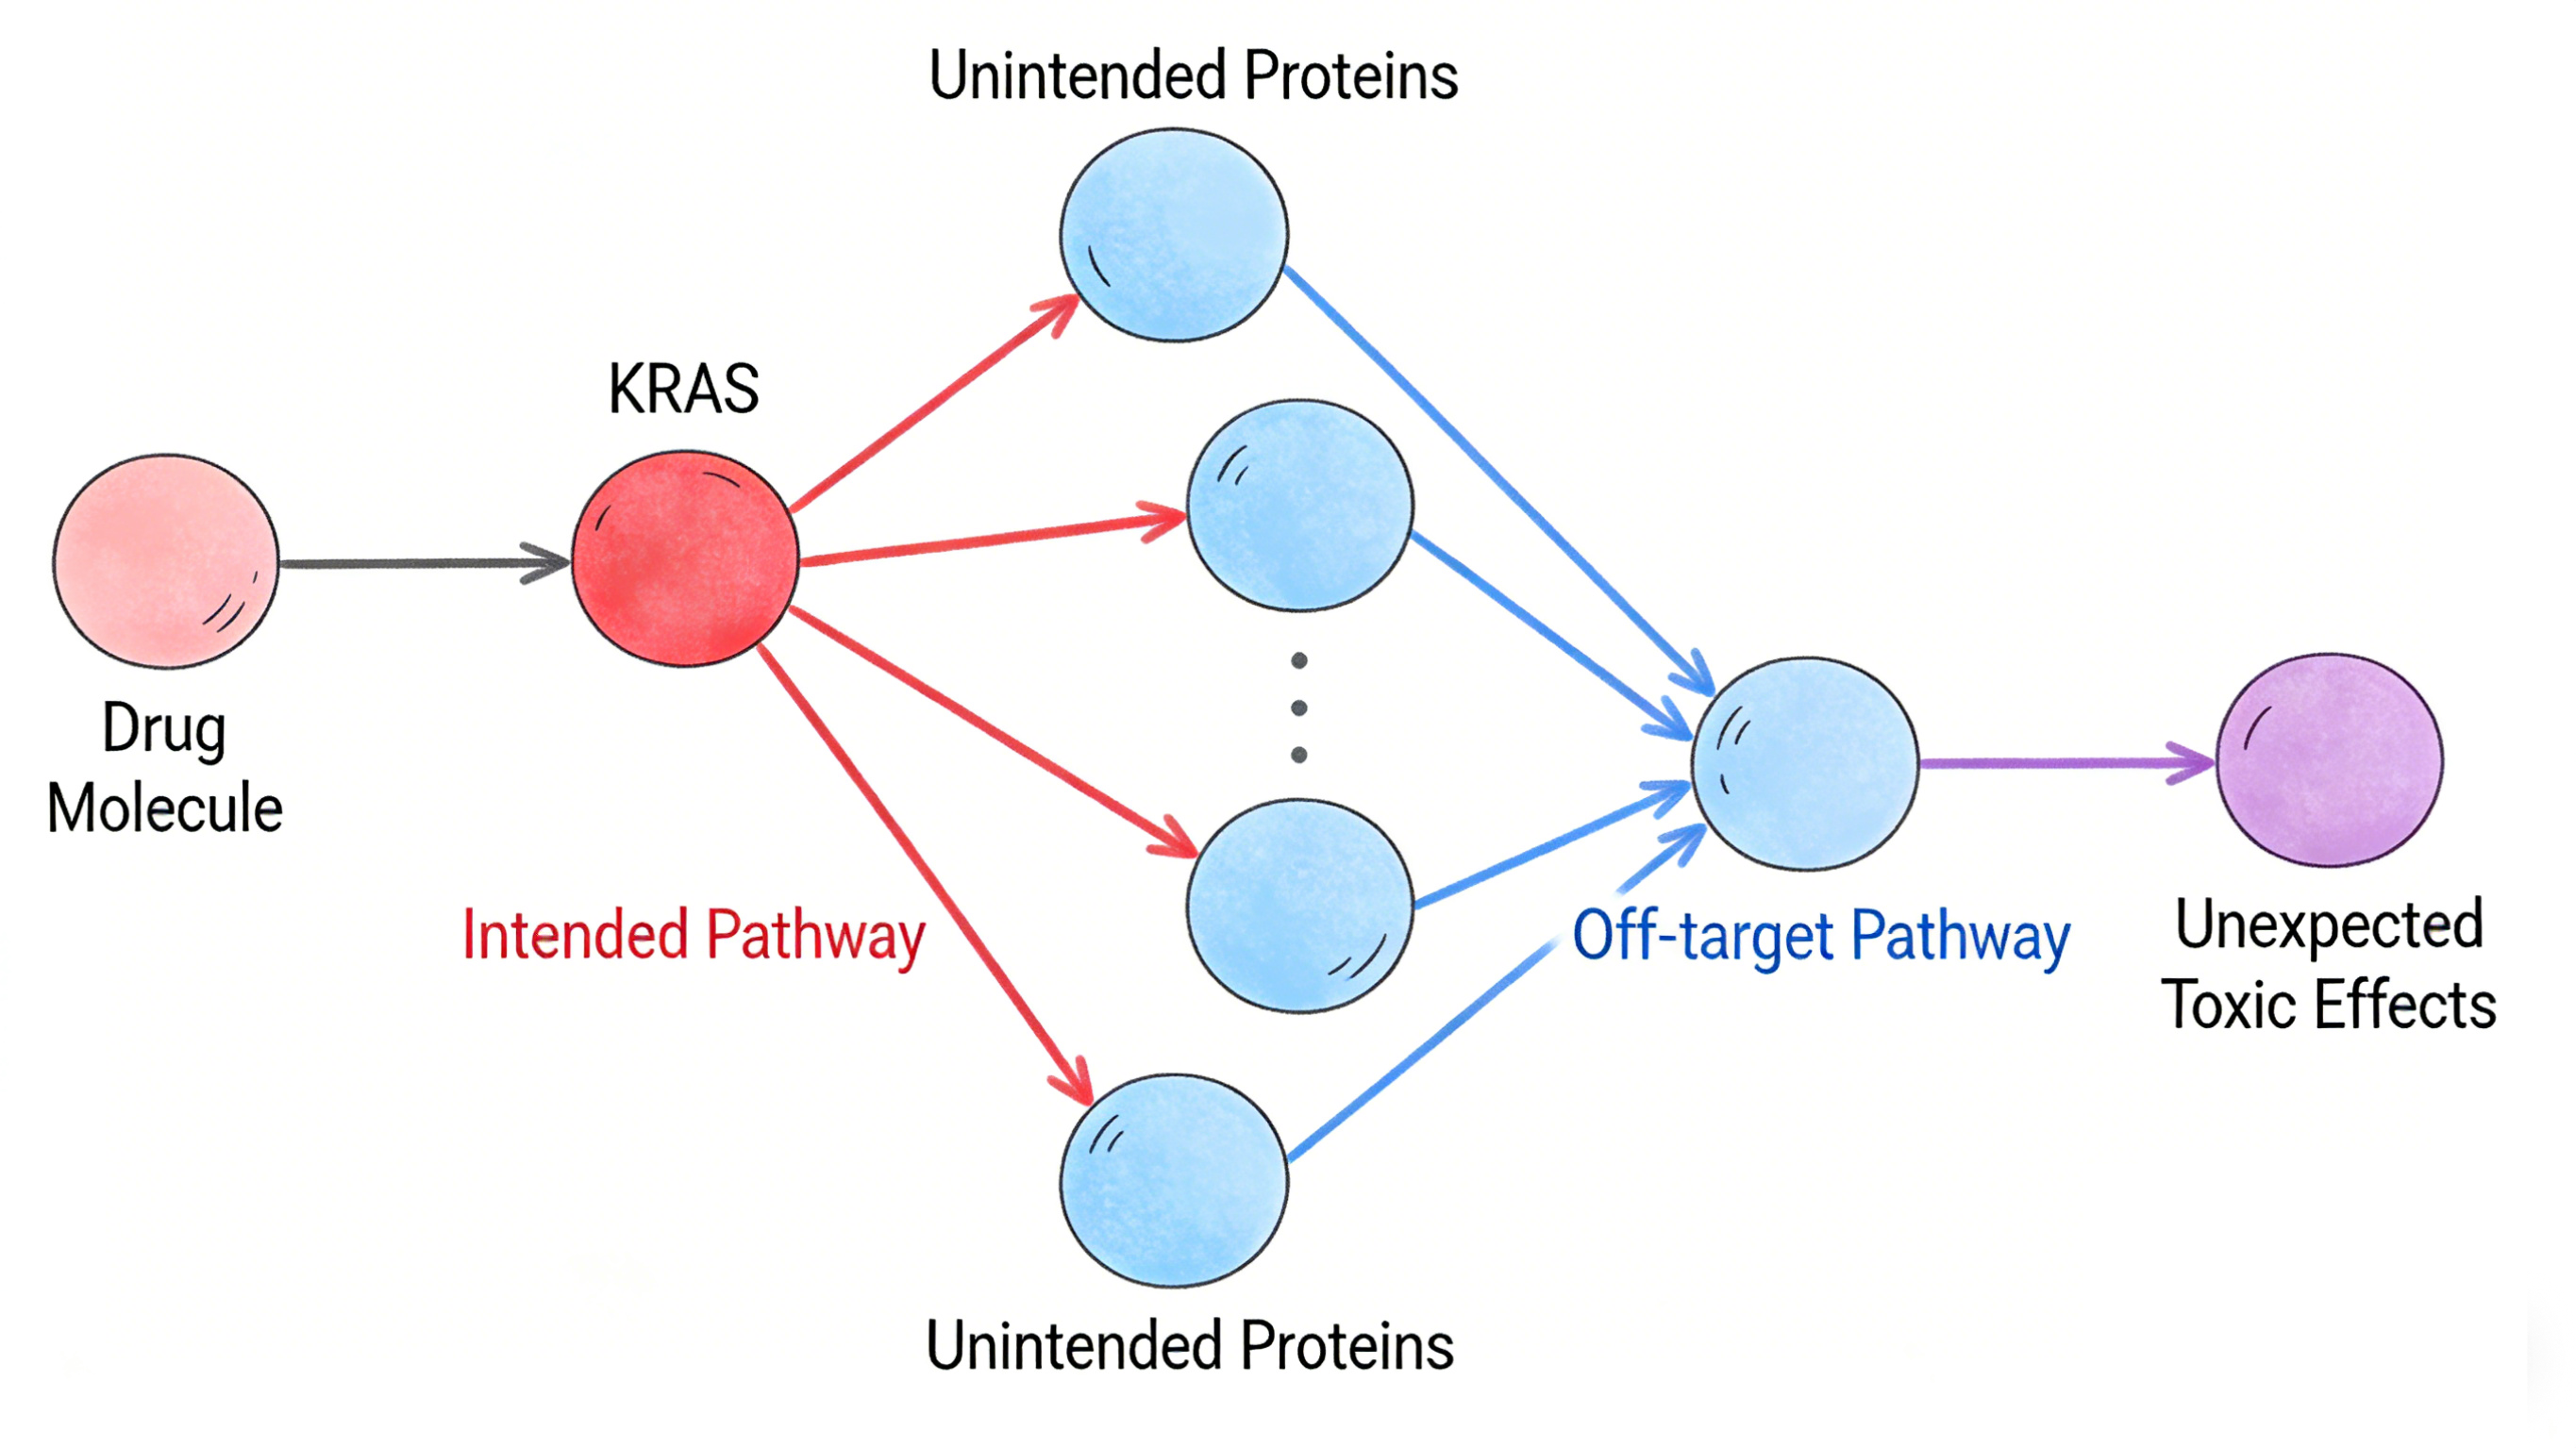
\includegraphics[width=\linewidth]{figures/compound_12_inhibitor_mechanism.png}
    \caption{Conceptual illustration of the AstraZeneca ``compound 12'' case. Although the compound targets KRAS, additional off-target effects may spread through molecular networks and cause unwanted outcomes.}
    \label{fig:compound_12_inhibitor_mechanism}
\end{figure}

\section{Drug perturbation}
Drug perturbation means using a drug to change the state of a cell so that the response can be studied. A drug usually starts by binding to one or more target proteins. This event may block a protein, activate it, or change its function in another way. The effect usually does not stop there. The signal can spread through molecular interactions inside the cell and affect many downstream genes.

\noindent In this thesis, the cellular response is described through gene expression. Gene expression shows how active each gene is. After drug treatment, some genes become more active and others become less active. Predicting these changes is useful because they give a broad summary of the molecular response in a form that can be measured at scale.

\section{High-throughput experiment}
\noindent Researchers use high-throughput experiments to study drug perturbations at scale. Figure~\ref{fig:well_plates} shows the basic setup. The idea is simple. Many cell lines are grown in multi-well plates. Many drugs are applied under controlled conditions. Gene expression is measured after treatment. This design makes it possible to compare many perturbations in a standard way.

\noindent This thesis uses the LINCS L1000 dataset. LINCS records gene expression responses for many compounds, cell lines, doses, and treatment times. Each well contains cells under one experimental condition. After treatment, the assay measures 978 landmark genes. The expression of additional genes can then be inferred from these measurements.

\noindent Each plate includes two main types of wells:
\begin{enumerate}
    \item \textbf{Treatment wells}: These contain cells exposed to a specific drug, usually dissolved in DMSO.
    \item \textbf{Control wells}: These contain cells exposed only to DMSO~\cite{Santos_2003}, without the active drug. They provide a reference for the same experimental setting without the drug effect.
\end{enumerate}

\noindent The key comparison is the difference between a treatment well and a matched control well. This comparison helps separate the drug effect from the background state of the cell. A control is useful only when it matches a comparable treatment condition. The dataset therefore records the cell line, drug dose, treatment time, and plate information. These variables matter because the same drug can act differently in different cell types and under different experimental settings.

\begin{figure}[!htbp]
    \centering
    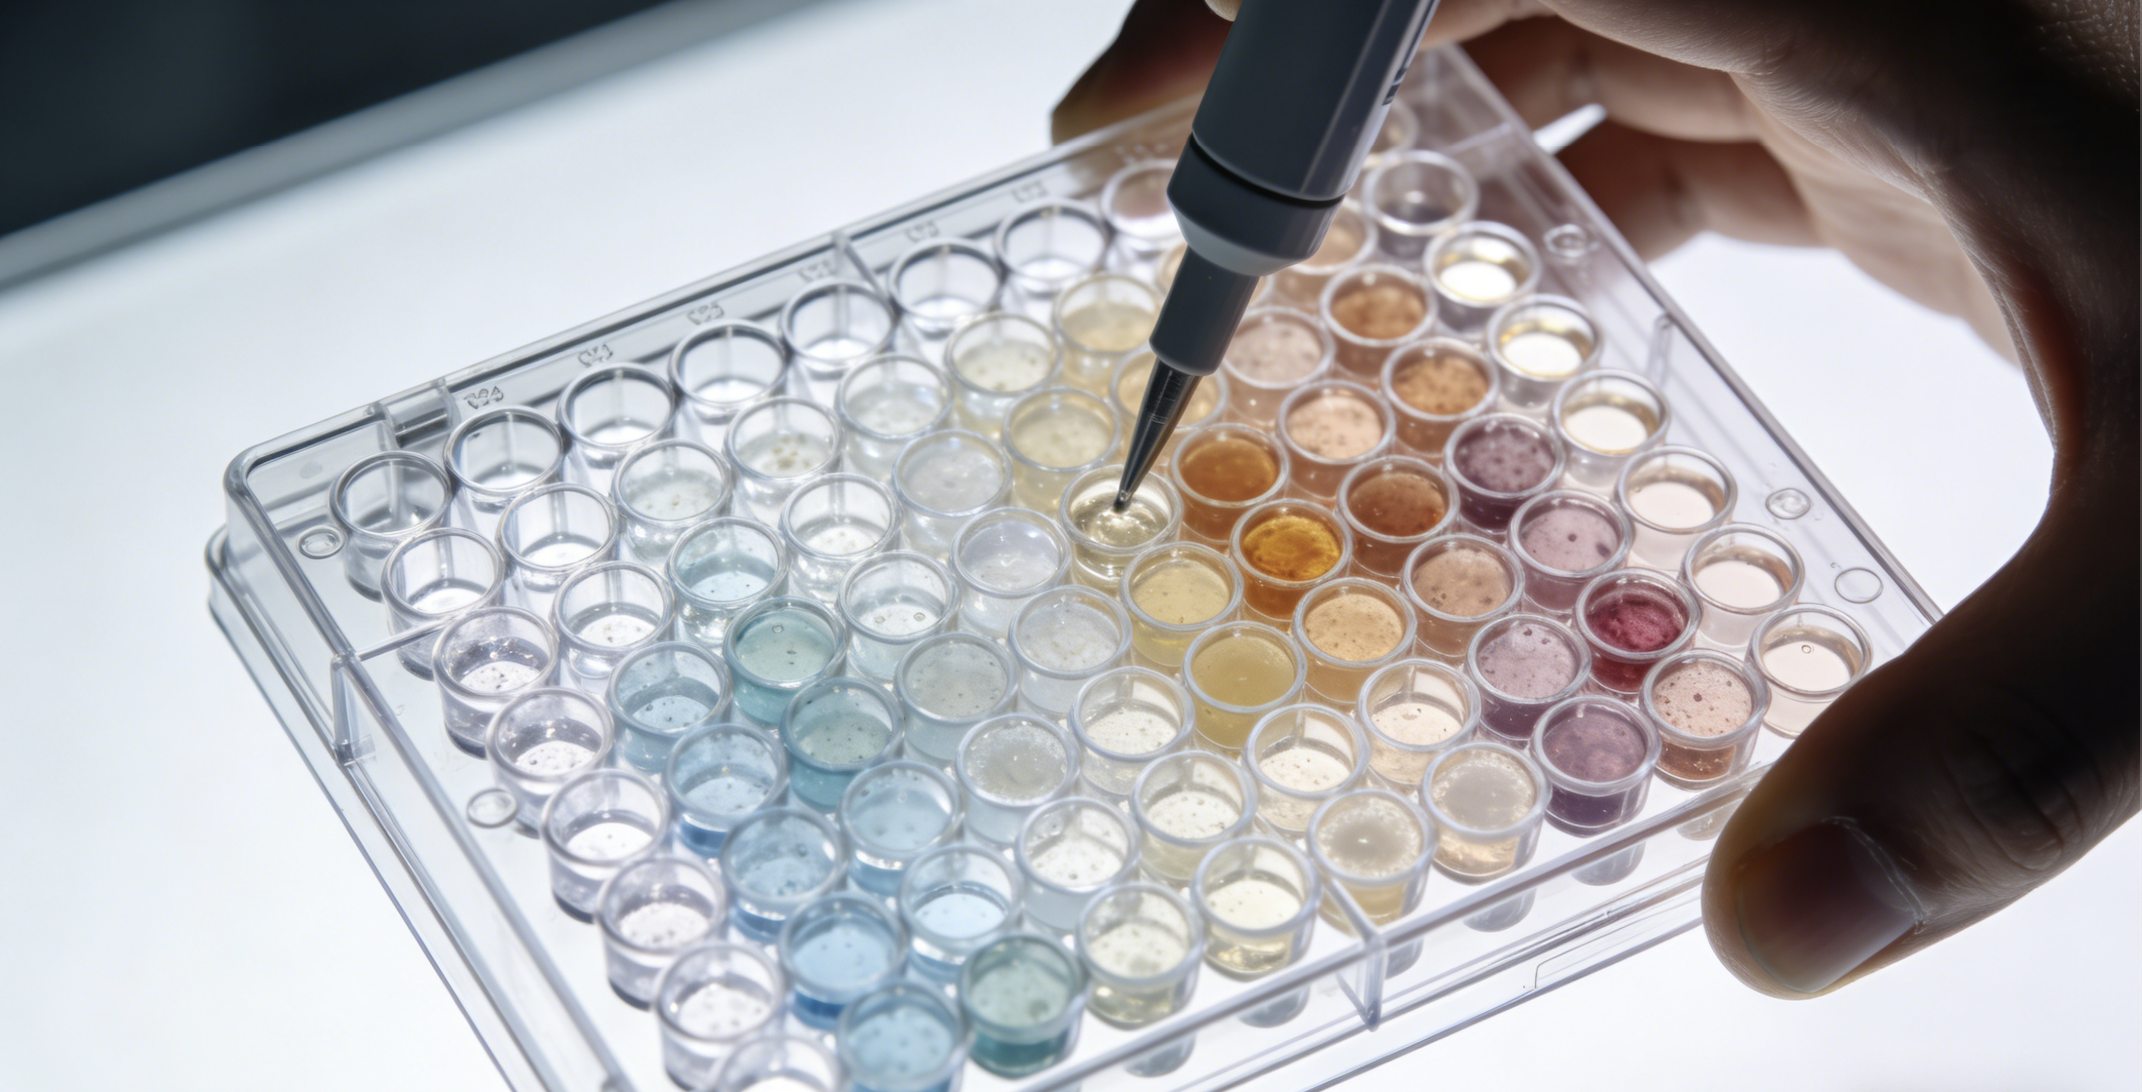
\includegraphics[width=\linewidth]{figures/well_plates.png}
    \caption{Sketch of the high-throughput well plate experiment, adapted from the LINCS L1000 assay description~\cite{l1000_paper}. A well is a small, separate container that holds cells for individual testing.}
    \label{fig:well_plates}
\end{figure}

\section{Prior knowledge of molecular interactions}

A second source of information comes from biological knowledge databases. These resources summarize known links among genes and proteins, such as regulation and signaling. This information is useful because drug effects do not come from one target alone. A drug may start from a small set of targets, but the response is shaped by how signals move through the surrounding molecular network.

\noindent OmniPath is one example of such a database. It integrates molecular interaction information from many curated resources and provides directed relationships that can be used to build a graph representation of the cell~\cite{turei2016omnipath}. In this thesis, the OmniPath network is aligned with the genes measured in LINCS L1000. This alignment places prior knowledge and experimental data in the same gene space.

\noindent This combination is central to the thesis. Perturbation data show what changes after treatment. The interaction network gives information about how those changes may spread through the cell. Drug target information marks where the perturbation begins. When these sources are combined, the model can make predictions that are more informed than predictions based on expression data alone.

\section{Aim}
This thesis studies how to predict gene expression changes after drug perturbation. The input includes the baseline state of the cell, known drug targets, and a molecular interaction network. The motivation is both practical and methodological. If such responses can be predicted more accurately, researchers can screen compounds more efficiently, prioritize follow up experiments, and better understand possible drug mechanisms.

\noindent The main idea is to combine two types of prior information. One is a molecular interaction network from a database such as OmniPath. The other is drug target information that marks where the perturbation begins. This thesis asks whether a graph based model can combine these sources to improve perturbation prediction.

The aims of this thesis are:
\begin{enumerate}
    \item To build a graph neural network (GNN) based on the OmniPath molecular interaction network. This model will predict drug-induced gene expression changes by combining baseline cell data and drug target information.
    \item To test how well the model works on unseen drugs and unseen cell lines (where test drugs or cells were never seen during training).
    \item To compare this model with baseline models that do not use a gene network, and to run tests to see how important the drug target information is.
\end{enumerate}

\noindent In our model, the graph represents molecular interactions, and the nodes correspond to the genes measured in the experiment. A graph attention network (GAT)~\cite{velickovic2018graph} is used because it can learn different weights for different neighbours. This is useful when the interaction graph is incomplete or noisy. The learned attention weights can also be inspected as an interpretation signal.

\begin{figure}[H]
    \centering
    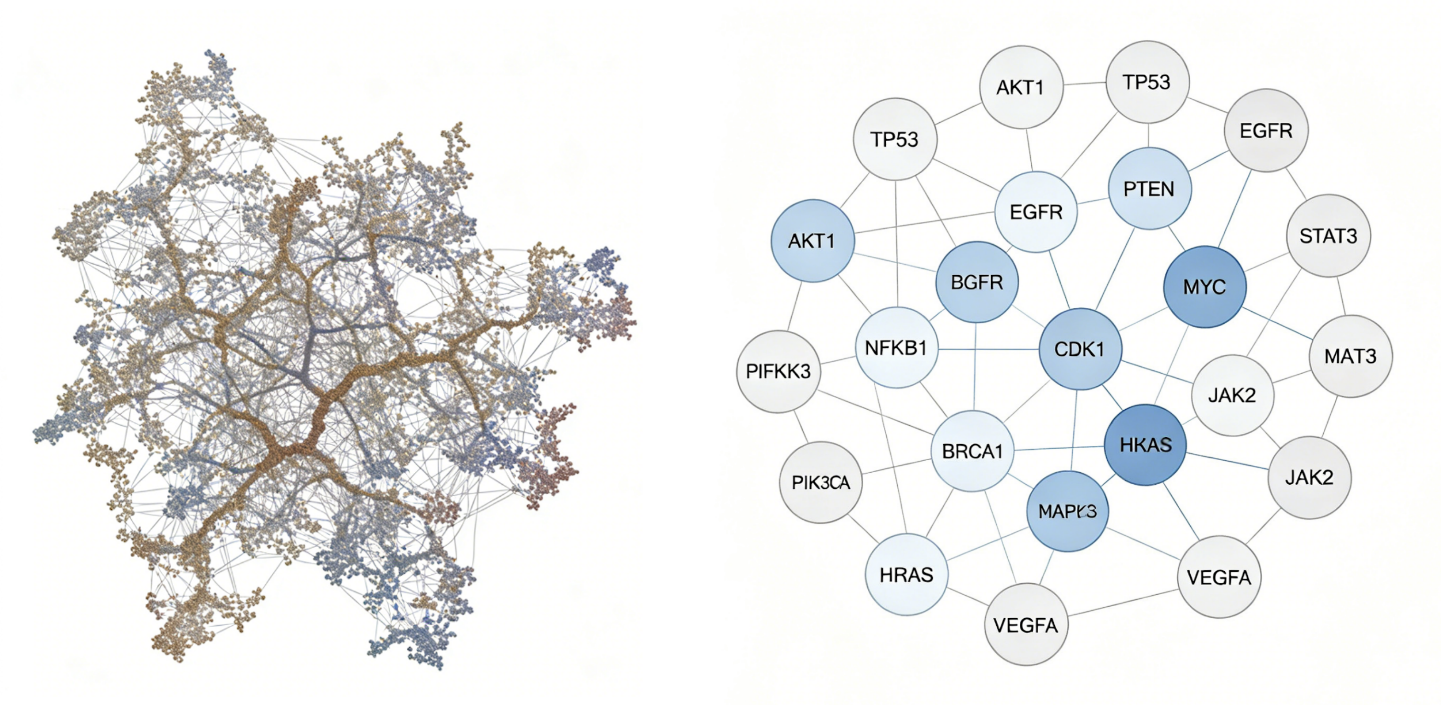
\includegraphics[width=\linewidth]{figures/gene_network_gnn_1.png}
    \caption{Left: Example of a real gene network, showing complex connections. Right: A simple drawing of a graph neural network (GNN), where genes and proteins are nodes, and their interactions are edges.}
    \label{fig:gene_network_gnn}
\end{figure}
\noindent Figure~\ref{fig:gene_network_gnn} gives a conceptual view of this modelling idea. The molecular network provides the graph structure, and the GNN uses this structure to propagate information from drug targets to downstream genes. The model is evaluated not only on random splits, but also on unseen drugs and unseen cell lines, so that generalization is tested under more realistic conditions.


\section{Related works}
Graph neural networks are now widely used in biology because many biological systems can be represented as graphs. A recent review summarizes GNN applications in single cell omics and discusses common architectures such as GCN, GraphSAGE, and GAT~\cite{li2025gnn_sc_review, scarselli2009gnn, kipf2017semi, hamilton2017inductive, velickovic2018graph}. These models are useful because each node can update its representation by using both its own features and information from connected neighbours. In biology, this makes them a natural choice for pathways, regulatory links, and other structured molecular systems.

\noindent Several studies have shown the value of graph based learning in perturbation biology. GEARS uses a gene relationship graph to predict responses to genetic perturbations in single cell data~\cite{roohani2023gears}. Cellograph models multi condition single cell datasets with graph based learning~\cite{shahir2024cellograph}. Evans et al. also study graph structured neural networks for perturbation biology more broadly~\cite{evans2024gsnn}. These studies focus on different data types and tasks, but they support the same basic idea. Graph structure can help connect an intervention to downstream molecular changes.

\noindent Another line of work predicts drug effects without an explicit biological interaction graph. Large resources such as LINCS L1000 and Connectivity Map make this possible because they provide gene expression responses for many compounds and cell lines~\cite{l1000_paper}. DeepCOP~\cite{woo2020deepcop} is one example. It uses a multilayer perceptron and drug information to predict gene regulation effects. This type of model is simple and scalable, and it provides a strong baseline. Still, it treats genes as separate outputs and does not use known molecular links among genes and proteins.

\noindent A different line of work uses prior biological knowledge more directly. Regulation Flow Analysis models how perturbation signals may move through a curated interaction network and uses this structure to infer possible mechanisms~\cite{roca2025rfa}. This kind of method is attractive because it is biologically interpretable. Its limit is that the propagation rule is largely fixed by the network and does not learn directly from large perturbation datasets. By contrast, data driven graph neural networks can learn how strongly information should move while still using the network structure.

\noindent Some recent studies combine graph structure with supervised prediction for drug response related tasks~\cite{wang2022graphgrp, kim2021gcn_drug_response}. These studies suggest that molecular networks can provide a useful inductive bias when labels are noisy or when the response follows many indirect molecular steps. They also show that graph quality matters. Curated resources such as OmniPath~\cite{turei2016omnipath} are therefore useful because they provide directed interactions and sign information for signal propagation.

\noindent Evaluation is also important in this area. Many studies report performance under random splits, where related drugs or cell contexts may appear in both training and test sets. For perturbation prediction, this can overestimate generalization. A stricter setting tests unseen drugs or unseen cell lines. This thesis follows that view and studies whether a graph based model can generalize beyond the conditions seen during training.

\section{Ethical considerations}
This thesis uses public data from LINCS L1000 and OmniPath. The data do not contain personal patient identifiers, and the work does not involve human or animal subjects. The main ethical concern is how the model outputs are used.

\noindent The model predicts gene expression changes after drug treatment. These predictions should be treated as computational hypotheses, not as evidence of efficacy or safety. They may support compound prioritization and hypothesis generation, but they should not be used for medical decision making without experimental and clinical validation.

\noindent Responsible reporting is therefore important. Model performance should be reported together with failure cases and limits of interpretation, especially when predictions are applied to unseen drugs or unseen cell lines.

\noindent Computational cost is another concern. Training deep learning models requires compute resources, and repeated hyperparameter search uses more energy. In this thesis, the models are trained on standard hardware with a limited set of configurations to keep resource use at a reasonable level.

\section{Limitations}
This study has limits from both the experimental data and the prior knowledge source. LINCS profiles are measured in a limited set of cell lines, and many of them are cancer derived. The results may therefore not transfer directly to primary cells or tissues. Experimental factors such as dose, treatment time, and plate context can also affect the measurements. Matched controls reduce some shared technical variation, but residual bias may remain.

\noindent OmniPath is built from published studies, and the available knowledge is uneven across pathways and genes. Well studied mechanisms tend to have more recorded interactions, while less studied mechanisms may be under represented. This imbalance can affect both prediction quality and interpretation.

\noindent The model also provides attention weights as an interpretation signal. These values show which edges receive stronger weight during message passing, but they do not prove biological causality. A highlighted path may fit known biology, and it may also reflect graph structure, data bias, or measurement noise.

\noindent Reproducibility is also an important practical issue. Model training includes random elements, so clear reporting of data splits, settings, and key hyperparameters is necessary for fair comparison and reliable interpretation.

% 数据来源补充说明
% LINCS L1000 数据集分为三个主要部分：
% GSE92742 (Phase I): Connectivity Map 基础，包含百万级基因表达谱，主要是小分子处理。
% GSE70138 (Phase II): 项目扩展，包含数十万表达谱，涵盖化学和遗传扰动（如基因过表达/敲除）。
% GSE92743 (Contest Data): 比赛测试集，答案隐藏用于算法评测。
% 本论文 trt/ctl 数据均来自上述数据集。
